% File: solutions/ex24.tex

\begin{soluzione}{24}
    \begin{enumerate}
        \item \textbf{Trasformata di Fourier di $x(t)$}
        
        Il segnale è un prodotto: $x(t) = g(t) \cdot m(t)$, dove:
        \begin{itemize}
            \item $g(t) = \left( \frac{\sin(\pi t)}{\pi t} \right)^2 = \text{sinc}^2(t)$. La sua trasformata, come suggerito, è una funzione triangolare: $G(f) = \text{tri}(f)$, che è un triangolo di altezza 1 e base da -1 a 1 Hz.
            \item $m(t) = 1 - 2\cos(2\pi t)$. La sua trasformata $M(f)$ si calcola usando la linearità e la trasformata notevole del coseno:
            \[
                M(f) = \delta(f) - 2 \cdot \frac{1}{2}[\delta(f-1) + \delta(f+1)] = \delta(f) - \delta(f-1) - \delta(f+1)
            \]
        \end{itemize}
        La trasformata $X(f)$ è la convoluzione $G(f) * M(f)$:
        \begin{align*}
            X(f) &= \text{tri}(f) * [\delta(f) - \delta(f-1) - \delta(f+1)] \\
            &= (\text{tri}(f) * \delta(f)) - (\text{tri}(f) * \delta(f-1)) - (\text{tri}(f) * \delta(f+1)) \\
            &= \mathbf{\text{tri}(f) - \text{tri}(f-1) - \text{tri}(f+1)}
        \end{align*}
        Questa espressione rappresenta un triangolo centrato in 0, a cui vengono sottratti due triangoli identici centrati in $\pm 1$ Hz.
        
        \item \textbf{Grafici di Modulo e Fase di $X(f)$}
        
        Analizziamo graficamente la sottrazione dei triangoli.
        \begin{itemize}
            \item In $|f| < 1$, $X(f) = \text{tri}(f) - \text{tri}(f-1) - \text{tri}(f+1) = (1-|f|) - (1-|f-1|) - (1-|f+1|)$. Poiché per $|f|<1$ si ha che $|f-1|=1-f$ e $|f+1|=f+1$, l'espressione diventa $(1-|f|) - (1-(1-f)) - (1-(f+1)) = (1-|f|) - f - (-f) = 1-|f|$. La parte centrale non viene modificata.
            \item In $1 \le |f| < 2$, si ha la coda del triangolo centrale a cui si sottrae un altro triangolo. Per $1 \le f < 2$, $\text{tri}(f)=0$, $\text{tri}(f-1)=1-(f-1)=2-f$, e $\text{tri}(f+1)=0$. Quindi $X(f) = -(2-f) = f-2$.
        \end{itemize}
        Per simmetria, per $-2 < f \le -1$, $X(f)=-f-2$.
        Lo spettro è quindi un triangolo centrale positivo e due triangoli negativi ai lati. Essendo una funzione reale, la fase sarà 0 dove $X(f)>0$ e $\pi$ (o $-\pi$) dove $X(f)<0$.
        
        \begin{center}
        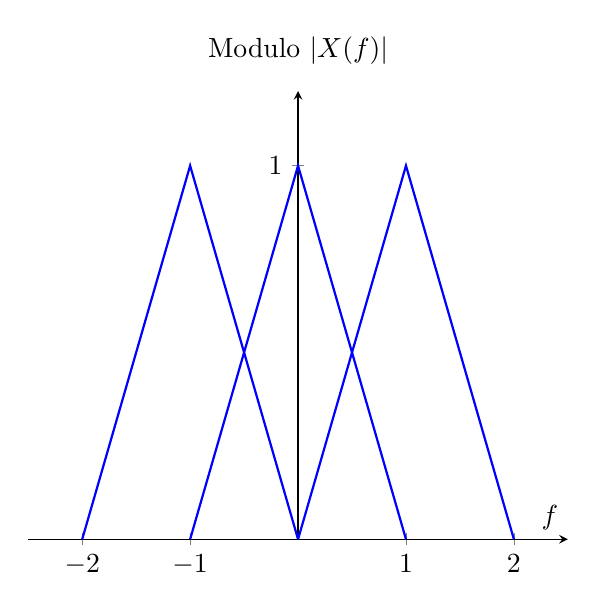
\begin{tikzpicture}
            \begin{axis}[
                title={Modulo $|X(f)|$},
                axis lines=middle, xlabel=$f$,
                xmin=-2.5, xmax=2.5, ymin=0, ymax=1.2,
                xtick={-2, -1, 0, 1, 2}, ytick={1}
            ]
            \addplot[blue, thick] coordinates {(-2,0) (-1,1) (0,0)};
            \addplot[blue, thick] coordinates {(0,0) (1,1) (2,0)};
            \addplot[blue, thick] coordinates {(-1,0) (0,1) (1,0)};
            \end{axis}
        \end{tikzpicture}
        \begin{tikzpicture}
            \begin{axis}[
                title={Fase $\angle X(f)$},
                axis lines=middle, xlabel=$f$,
                xmin=-2.5, xmax=2.5, ymin=-4, ymax=4,
                xtick={-2, -1, 0, 1, 2}, ytick={-3.14, 0, 3.14},
                yticklabels={$-\pi$, 0, $\pi$}
            ]
            \addplot[red, thick] coordinates {(-2.5, 3.14) (-2, 3.14)};
            \addplot[red, thick, dotted] coordinates {(-2,0) (-2,3.14)};
            \addplot[red, thick] coordinates {(-2, 0) (-1, 0)};
            \addplot[red, thick, dotted] coordinates {(-1,0) (-1,3.14)};
            \addplot[red, thick] coordinates {(-1, 3.14) (1, 3.14)};
            \addplot[red, thick, dotted] coordinates {(1,0) (1,3.14)};
            \addplot[red, thick] coordinates {(1,0) (2,0)};
            \addplot[red, thick, dotted] coordinates {(2,0) (2,3.14)};
            \addplot[red, thick] coordinates {(2,3.14) (2.5,3.14)};
            \end{axis}
        \end{tikzpicture}
        \end{center}
        
        \item \textbf{Spettro del Segnale Ricostruito $X_R(f)$}
        
        La banda del segnale è $B=2$ Hz. La frequenza di campionamento è $f_s=3$ Hz.
        La condizione di Nyquist ($3 \ge 2 \cdot 2$) è violata, quindi c'è aliasing.
        La banda base di ricostruzione è $[-f_s/2, f_s/2] = [-1.5, 1.5]$ Hz.
        
        Dobbiamo sommare le repliche di $\tilde{X}(f)$ che cadono in questa banda. Oltre alla replica centrale ($k=0$), dobbiamo considerare le code delle repliche centrate a $\pm f_s = \pm 3$ Hz.
        
        Il contributo della replica $k=0$ in $[-1.5, 1.5]$ è $X(f) = \text{tri}(f) - \text{tri}(f-1) - \text{tri}(f+1)$.
        
        Il contributo della replica $k=1$ (centrata a 3 Hz) in $[-1.5, 1.5]$ è $X(f-3)$. Questa è non nulla per $f-3 \in [-2, 2]$, cioè $f \in [1, 5]$. La sovrapposizione è nell'intervallo $[1, 1.5]$.
        
        Il contributo della replica $k=-1$ (centrata a -3 Hz) in $[-1.5, 1.5]$ è $X(f+3)$, non nulla per $f \in [-5, -1]$. La sovrapposizione è in $[-1.5, -1]$.
        
        Lo spettro campionato con aliasing, $\tilde{X}_{aliased}(f)$, nella banda base è:
        \[
            \tilde{X}_{aliased}(f) = X(f) + X(f-3) + X(f+3) \quad \text{per } |f| \le 1.5
        \]
        Il filtro di ricostruzione $H_R(f)$ ha guadagno $T=1/3$ e taglia a $\pm 1.5$ Hz.
        Lo spettro ricostruito $X_R(f) = \tilde{X}_{aliased}(f) \cdot (1/f_s)$.
        
        Analizziamo il risultato. Per $1 \le f \le 1.5$:
        \begin{align*}
            X(f) &= f-2 \\
            X(f-3) &= (1-|f-3|) - \dots = 1-(3-f) = f-2 \\
            \tilde{X}_{aliased}(f) &= (f-2) + (f-2) = 2f-4
        \end{align*}
        Per simmetria, per $-1.5 \le f \le -1$, $\tilde{X}_{aliased}(f) = -2f-4$.
        Per $|f|<1$, non c'è sovrapposizione, quindi $\tilde{X}_{aliased}(f)=X(f)=1-|f|$.
        
        Moltiplicando per $1/f_s=1/3$, otteniamo $\mathbf{X_R(f)}$:
        \[
            X_R(f) = \frac{1}{3} \begin{cases} -2f-4 & \text{per } -1.5 \le f \le -1 \\ 1-|f| & \text{per } |f|<1 \\ 2f-4 & \text{per } 1 \le f \le 1.5 \\ 0 & \text{altrimenti} \end{cases}
        \]
    \end{enumerate}
\end{soluzione}